\chapter{Applications} \label{chap:App}

\section{Risks measures}

In this section we discuss different ways to measure the risk of portfolio.


\begin{definition}
	A portfolio with $n$ assets, $A_1, A_2, \dots, A_n$, is a vector $x^\top = (x_1, x_2, \dots, x_n)\in \R^n$ where each coordinate $x_i$ is the weight of capital invested in asset $A_i$.
\end{definition}

Let $L(x,y)$ be the loss associated with the decision vector $x$, to be chosen from a certain subset $X$ of $\R^n$ and the random vector $y \in \R^m$. The vector $x$ can be interpreted as representing a portfolio, with $X$ as the set of available portfolios
(subject to various constraints). The vector $y$ stands for the uncertainties, e.g. in market parameters, that can affect the loss. Of course the loss might be negative and thus, in effect, constitute a gain.

For each $x$, the loss $L(x,y)$ is a random variable having a distribution in $\R$ induced by that of $y$. The underlying probability distribution of $y \in \R^m$ will be assumed to have density, which we denote by $p(y)$.

The probability of $f(x,y)$ not exceeding a threshold $\alpha$ is given then by
\[
	\Psi (x,\alpha) = \int_{L(x,y)\leq \alpha} p(y)\,dy.
\]
As a function of $\alpha$ for fixed $x, \Psi(x, \alpha)$ is the \textit{cumulative distribution function} for the loss associated with $x$. Since $p(y)$ is continuous, $\Psi(x, \alpha)$ is nondecreasing with respect to $\alpha$ and continuous.


The \textit{expected loss} $\mu$ of a portfolio $x$ is given by
\[
	\mu(x) = \int_{\R} L(x,y)\,p(y)\,dy.
\]
Moreover, the \textit{loss variance} of $x$ is
\[
	\sigma^2(x) = \int_{\R} \big(L(x,y)-\mu(x)\big)^2\,p(y)\,dy
\]
and the \textit{volatility} of the loss is $\sigma(x)$.

The volatility of the loss was defined as a \textit{risk measure} to a portfolio by Nobel laureate in economics, Harry Markowitz in 1952 (see in \cite{Markowitz1952}) under the hypothesis of loss has a normal distribution. In the following we see that this choice is not the better one.

In 1999 Artzner, Delbaen, Eber and Heath (see in \cite{Artzner1999}) defined, what they called \textit{coherent risk measure}, from the following axioms to a risk measure $\mathcal{R}$:

\begin{axiom}[Translation invariance] For all portfolio $x$ and all $m\in\mathbb{R}$,  we have
	\[
		\mathcal{R}(x+m) = \mathcal{R}(x)-m.
	\]
\end{axiom}
This means that adding an amount of cash, $m$, to a portfolio decreases your risk by the same amount.

\begin{axiom}[Subadditivity] If $x_A$ and $x_B$ are two portfolios, then
	\[
		\mathcal{R}(x_A+x_B) \leq \mathcal{R}(x_A) + \mathcal{R}(x_B),
	\]
\end{axiom}
In particular, this property means that ``a merger does not create extra risk.''

\begin{axiom}[Positive homogeneity] For all portfolio $x$ and all $\lambda\leq 0$ we have
	\[
		\mathcal{R}(\lambda x) = \lambda \mathcal{R}(x), \qquad \mbox{se } \lambda
		\geq 0.
	\]
\end{axiom}
This property implies that the risk measure is a linear function of the size of the position.

\begin{axiom}[Monotonicity] Let $x_A$, $x_B$ be two portfolios,
	\[
		\mbox{if } x_A \prec x_B, \quad \mbox{then } \quad \mathcal{R}(x_A) \geq \mathcal{R}(x_B).\\
	\]
\end{axiom}
If a portfolio $x_A$ performs worse than $x_B$ in any
scenario $(x_A \prec x_B)$, then it means that the portfolio $x_A$ is
riskier than $x_B$.

\begin{definition}
	A risk measure satisfying the axioms of translation invariance, subadditivity, positive homogeneity, and monotonicity is called \textbf{coherent}.
\end{definition}


When the risk measure is not assumed to have variations proportional to the risk variations themselves, the positive homogeneity is no longer satisfied. Alternative axioms can be proposed.

\begin{axiom}[Convexity] For all portfolios $x_A$, $x_B$ and for all $0\leq \lambda \leq 1$,
	\[
		\mathcal{R}(\lambda x_A + (1-\lambda)x_A) \leq \lambda \mathcal{R}(x_A) + (1-\lambda) \mathcal{R}(x_B).
	\]
\end{axiom}

This axiom  was proposed in 2002 by Föllmer and Shield (see in \cite{Follmer2002}). It means that diversification does not increase risk.

\begin{definition}
	A risk measure satisfying the axioms of translation invariance, monotonicity, and convexity is called \textbf{convex}.
\end{definition}

\begin{proposition}
	A convex risk measure is coherent if it satisfies the positive homogeneity. Note also that the positive homogeneity and the subadditivity implies the convexity.
\end{proposition}

The standard deviation does not satisfy translation invariance, however, this condition was defined with the perspective of banking system risk and is often ignored in case of portfolio construction.

In financial business, some of the risk management requirements are done in terms of loss distribution percentiles. An upper percentile of the loss distribution is called \textit{Value-at-Risk} ($\mbox{VaR}_\beta$)\footnote{By definition, $\mbox{VaR}_\beta$ is the percentile of the loss distribution, i.e., with a specified confidence level $\beta$, the $\mbox{VaR}_\beta$ of a portfolio is the lowest amount $\zeta$ such that, with probability $\beta$, the loss is less or equal to $\zeta$.}. For instance, $\mbox{VaR}_{0.95}$ is an upper estimate of losses which is exceeded with 5\% probability. The popularity of $\mbox{VaR}_\beta$ is mostly related to a simple and easy to understand representation of high losses. $\mbox{VaR}_\beta$ can be quite efficiently estimated and managed when underlying risk factors are normally (log-normally) distributed.

An alternatuve measure of losses is another percentile risk measure which is called \textit{Conditional Value-at-Risk} ($\mbox{CVaR}_\beta$). The $\mbox{CVaR}_\beta$ risk measure is closely related to $\mbox{VaR}_\beta$. For continuous distributions, $\mbox{CVaR}_\beta$ is defined as the conditional expected loss under the condition that it exceeds $\mbox{VaR}_\beta$, see Rockafellar and Uryasev (see \cite{RockafellarUryasev2001}). For continuous distributions, this risk measure also is known as \emph{Expected Shortfall}, \textit{Mean Excess Loss}, \textit{Mean Shortfall}, or \textit{Tail Value-at-Risk}.


\begin{figure}[H]
	\centering
	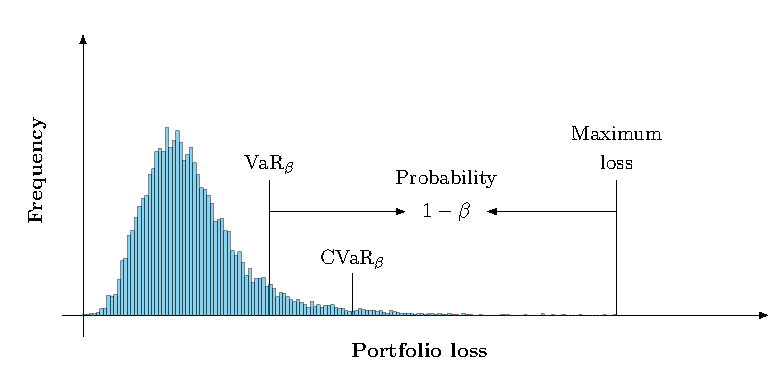
\includegraphics{figures/VarCvar.pdf}
	\caption{Portfolio Loss Distribution, VaR and CVaR}
	\label{fig:VarCvar}
\end{figure}

\begin{remark}\normalfont \hspace{1cm}
	\begin{itemize}
		\item The $\mbox{VaR}_\beta$ answers the question: what is the maximum loss with a specified confidence level $\beta$?
		\item The $\mbox{CVaR}_\beta$ answers the following question: what is the average loss in the $100(1-\beta)$\% worst case scenarios?
	\end{itemize}
\end{remark}

The $\mbox{VaR}_\beta$ and $\mbox{CVaR}_\beta$ values for the loss random variable $L(x,y)$ associated with $x$ and any specified probability level $\beta \in (0,1)$ will be denoted by $\alpha_\beta(x)$ and $\mbox{ES}_\beta(x)$. In our setting they are given by
\begin{equation}\label{eq:var}
	\alpha_\beta(x) = \min\{\alpha\in\mathbb{R} : \Psi(x,\alpha)\geq \beta \},
\end{equation}
and
\begin{equation}\label{eq:cvar}
	\mbox{ES}_\beta(x) = \frac{1}{1-\beta}\int_{L(x,y)\geq \alpha_\beta(x)} L(x,y)\, p(y)\,dy
\end{equation}

Although $\mbox{VaR}_\beta$ is a very popular measure of risk, $\mbox{VaR}_\beta$ is not a coherent risk measure as it does not satisfy subadditivity. 
 














\begin{remark}\normalfont \hspace{1cm}
	\begin{itemize}
		\item The standard deviation does not satisfy condition 4, however, this condition was defined with the perspective of banking system risk and is often ignored in case of portfolio construction.
		\item VaR is not a coherent risk measure as it does not satisfy condition 1. This is a problem because the portfolio’s risk may have be meaningful in this case.
		\item CVaR is a coherent risk measure.
	\end{itemize}
\end{remark}


Let us now assume that the returns are normally distributed, that is, $R\sim N(\mu,\sigma^2)$, where $\mu(x)=x^\top\mu$ and
$\sigma(x)=\sqrt{x^\top \Sigma x}$. Let $\phi(z) = \frac{1}{\sqrt{2\pi}}e^{-z^2/2}$ be the probability density function of Standard Normal Distribution and $\Phi(x) = \int_{-\infty}^{x}\phi(z) dz$
the standard normal accumulated density function.

By definition we have
$P\Big[L(x)\leq \mbox{VaR}_\alpha(x)\Big]=\alpha$, so
$P\Big[R(x)\leq -\mbox{VaR}_\alpha(x)\Big]=1-\alpha$, which standardizing
we have:
\[
	P\left[ \frac{R(x)-x^\top\mu}{\sqrt{x^\top \Sigma x}} \leq \frac{-\mbox{VaR}_\alpha(x)- x^\top\mu}{\sqrt{x^\top \Sigma x}}
		\right]=1-\alpha.
\]
Hence,
\[
	\frac{-\mbox{VaR}_\alpha(x)-x^\top\mu}{\sqrt{x^\top \Sigma x}}=\Phi^{-1}(1-\alpha)
\] and since $\Phi^{-1}(\alpha)=-\Phi^{-1}(1-\alpha)$, we have
\begin{equation}\label{eq:var2}
	\mbox{VaR}_\alpha(x)=-x^\top\mu+ \Phi^{-1}(\alpha)\sqrt{x^\top \Sigma x}.
\end{equation}

This is a special case of the standard deviation-based risk measure with $c = \Phi^{-1} (\alpha)$. It implies that the value-at-risk is a coherent and convex risk measure if the asset returns are normally distributed. The expression of the expected shortfall is:

\[
	\mbox{ES}_\alpha(x) = \frac{1}{1-\alpha}\int_{\mbox{VaR}_\alpha(x)}^\infty u p(u)du,
\] considering $p(u)$ the normal density function, we have that:
\[
	\mbox{ES}_\alpha(x) = \frac{1}{1-\alpha}\int_{-\mu(x)+ \sigma(x)\Phi^{-1}(\alpha)} ^\infty \frac{u}{\sigma(x)\sqrt{2\pi}} e^{-\frac{1}{2}\Big(\frac{u+\mu(x)}{\sigma (x)}\Big)^2} du,
\]

With the variable change
$t=\frac{u+\sigma(x)}{\sigma(x)}$, we obtain

\[
	\begin{aligned}
		\mbox{ES}_\alpha(x) & = \frac{1}{1-\alpha}\int_{\Phi^{-1}(\alpha)}^\infty (-\mu(x)+ \sigma(x)t) \frac{1}{\sqrt{2\pi}} e^{-t^2/2}dt \\
		                    & = -\frac{\mu(x)}{1-\alpha}[\Phi(t)]_{\Phi^{-1}(\alpha)}^\infty +
		\frac{\sigma(x)}{(1-\alpha)\sqrt{2\pi}}\int_{\Phi^{-1}(\alpha)}^\infty t e^{-t^2/ 2}dt                                             \\
		                    & =-\mu(x) + \frac{\sigma(x)}{(1-\alpha)\sqrt{2\pi}}\Big[-e^{-t^2/2} \Big] _{\Phi^{-1}(\alpha)}^\infty         \\
		                    & = -\mu(x) + \frac{\sigma(x)}{(1-\alpha)\sqrt{2\pi}}e^{-\frac{[\Phi^{-1}(\ alpha)]^2}{2}}
	\end{aligned}.
\]

So CVaR can be calculated by
\begin{equation}\label{eq:cvar2}
	\mbox{ES}_\alpha(x)=-x^\top \mu + \frac{\phi(\Phi^{-1}(\alpha))}{1-\alpha}\sqrt{x^ \top \Sigma x}.
\end{equation}
Like the value-at-risk, it is a standard deviation-based risk measure with $c ={\phi(\Phi^{-1}(\alpha))}/{(1-\alpha)}$
In the Gaussian world, different risk measures can be calculated using the expected return and volatility. Note by (\ref{eq:var2}) and (\ref{eq:cvar2}), that both Var and CVaR are the form $-\mu(x)+c\sigma(x)$. In general, we want a portfolio with positive returns, that is, $\mu(x)\geq0$. If the portfolio manager has very optimistic forecasts, component $\mu(x)$ may substantially reduce the risk measure. This explains why omitting the mean component is standard practice in the asset management industry.

\begin{example}\normalfont
	We consider three stocks $A$, $B$ and $C$ whose current prices are respectively $\$ 15.00$, $\$ 25.00$ and $\$ 30.00$. We assume that their expected returns are equal to $30$ bps\footnote{1 bps or one basis point is equivalent to
		0.01\% (the hundredth part of 1\%) or 0.0001 in decimal form.}, $50$ bps and $20$ bps on a daily basis and their daily volatilities are $3\%$, $2\%$, and $1\%$ respectively. The asset correlation matrix is given by
	\[
		\rho = \left(
		\begin{array}{rrr}
				1.00 & 0.40 & 0.15 \\
				0.40 & 1.00 & 0.60 \\
				0.15 & 0.60 & 1.00
			\end{array}
		\right)
	\]

	We consider a portfolio composed by $100$ stocks $A$, $200$ stocks $B$ and $100$ stocks $C$. The value of this portfolio is $\$ 9,500.00$, being $\$ 1,500.00$ invested in stock $A$, $\$ 5,000.00$ in stock $B$ and $\$ 3,000.00$ in stock $C$, therefore the weights of the stocks in this portfolio are $15.79\%$, $52.63\%$, and $31.58\%$ respectively, so $x=(0.1579;\;0.5263;\; 0.3158)$. The expected return on the portfolio is $\mu(x) = 30\times0.1579+50\times0.5263+20\times0.3158$, that is, $\mu(x) = 37$ bps. Using the relationship $\Sigma_{i,j}=\rho_{i,j}\sigma_1\sigma_j$ we find the covariance matrix
	\[
		\Sigma = \left(
		\begin{array}{llr}
				9.0 & 2.4 & 4.5 \\
				2.4 & 4.0 & 1.2 \\
				4.5 & 1.2 & 1.0
			\end{array}
		\right)\times10^{-4},
	\] since the volatility of portfolio is given by $\sigma^2(x) = x^\top \Sigma x$, we have that $\sigma(x) = 1.51\%$.

	Considering $\alpha = 0.99$, we have $\Phi^{-1}(0.99) = 2.325$ and
	$\phi(\Phi^{-1}(0.99))=\phi(2.325)=2.68\%$. Using the equations
	$(\ref{eq:var2})$ and $(\ref{eq:cvar2})$ we have

	\[
		\begin{aligned}
			\mathrm{VaR}_{99\%}(x) & = -0.37\% + 2.325 \times 1.51\% = 3.14\%              \\
			\mathrm{ES}_{99\%}(x)  & = -0.37\% + \frac{2.68}{0.01} \times 1.51\% = 3.68\%.
		\end{aligned}
	\]

	Risk can also be expressed in monetary terms, in this case,

	\[
		\begin{aligned}
			\mathrm{VaR}_{99\%}(x) & = 3.14\% \times \$ 9,500.00 = \$ 298.30  \\
			\mathrm{ES}_{99\%}(x)  & = 3.68\% \times \$ 9,500.00 = \$ 349.60.
		\end{aligned}
	\]
	According to the result of {\rm VaR}, in $99\%$ of the days, the loss will be less than $\$ 298.30$, however in the $1\%$ of the remaining days the {\rm VaR} does not measure how much great can be the loss, this is the role of {\rm CVaR} which indicates that the average loss will be $\$ 349.60$ on the worst $1\%$ days.
\end{example}





\section{The Gaussian Case}

\section{Case Study}